\documentclass[a4paper, 11pt]{article}
\usepackage{hyperref}
\voffset -0cm
\hoffset 0.0cm
\textheight 23cm
\textwidth 16cm
\topmargin 0.0cm
\oddsidemargin 0.0cm
\evensidemargin 0.0cm

\usepackage{epsfig}
\usepackage{setspace}
\usepackage{fancyheadings}
\usepackage{amsmath}
\usepackage{amssymb}
\usepackage{graphicx}
\usepackage{url}

\title{}
\author{}
\date{}

\begin{document}

\begin{center}
	\LARGE \textbf{TD9: Voronoi Map/Distance Transformation via Jump Flooding}
\end{center}

\bigskip
\par In this TP, the idea is to implement a Voronoi map algorithm called \emph{jump flooding algorithm} (JFA). This algorithm is not exact in the sense that it may contains errors and is not optimal in terms of computational cost. However, it has several properties which makes it useful in some applications.



% -------------------------------------------------------
\section*{Exercise 1 \rm Jump Flooding Algorithm}

{\bf Warm up} Create a DGtal program which constructs an image with $-1$  values everywhere and a positive  values at some random sites (one value per site, this value will be used to characterize each site). The generating function is thus parameterized by $n$, the image width, and $N$ the number of sites. Here is an example of image management in DGtal
\begin{verbatim}
  #include <DGtal/helpers/StdDefs.h>
  #include "DGtal/images/ImageContainerBySTLVector.h"
  ...
  //Image type (with unsigned int values)
  typedef ImageContainerBySTLVector< Domain, int > Image;

  //Create an image [0,n]x[0,n]
  Image myImage( Domain ( Point(0,0), Point(n,n)));

  //Get and Set value
  myImage.setValue( Point(2,3), 42);
  int val = myImage( Point(2,3) );  //val == 42

  //Decide if a point is in the image domain
  bool res = myImage.domain().isInside( Point(17,17) ); //res==true if n>=17

  //Iterate on image values
  for(Image::Domain::ConstIterator it = myImage.domain().begin(),
      itend = myImage.domain().end(); it!=itend ; +=it) {
     int val2 = myImage( *it );
     std::cout << val2 <<" ";
  }
\end{verbatim}


\par The \emph{JFA of step $k$} (denoted $JFA(k)$) is defined as follow. For each point $p=(x,y)$ in the image:
	\begin{itemize}
	\item Collect the four sites stored in the image at pixels $S$
          with  $l_\infty$  distance $k$. More precisely, $S=\{ (x \pm k,y\pm k)\}$.
	\item Compute the distance (using $l_2$ metric) between $p$ and all sites (eight sites in $S$ and the site stored at $p$)
	\item Store the site with closest distance at $p$ in the image.
	\end{itemize}

\noindent When probing the site at coordinate $(x,y)$, if you get a $-1$ value or if you jump outside the image, consider that the distance is $+\infty$.

\bigskip
{\bf Questions:}
\begin{itemize}
	\item Implement the $JFA(k)$ method. You can use a Board export to display the Voronoi diagram under construction (cf Fig. 1) and the following code snippet (assuming that $voro$ is the name of your image).
\begin{verbatim}
  board.clear();
  board << voro.domain();
  for(typename Image::Domain::ConstIterator it =voro.domain().begin(),
           itend = voro.domain().end(); it != itend; ++it) {
    if (voro( *it ) != -1) {
      //random color from site index voro( *it )
      unsigned char color = (unsigned char) (voro( *it )*13727 % 256);
      board << CustomStyle( (*it).className(), new CustomColors(Color(c,c,c),Color(c,c,c)))
            << (*it);;
    }
  }
  board.save....
\end{verbatim}
	\item What is the computational cost of one JFA step ?
	\item The overall JFA algorithm consist in JFA(k) steps with $k=\{\frac{n}{2}, \frac{n}{4}, \ldots, 1\}$ (see Fig. 1). Sometimes, we consider a $JFA+1$ in which the last step ($k=1$) is performed twice. What is the overall complexity of such algorithm ?
	\item Implement the JFA algorithm.
	\item Implement the exact "brute force" Voronoi map algorithm (for each point, scan all sites and store the closest). Compare the result and return the average distance error.
	\item From the JFA Voronoi map, output the distance transformation.
\end{itemize}

\begin{figure}
  \centering  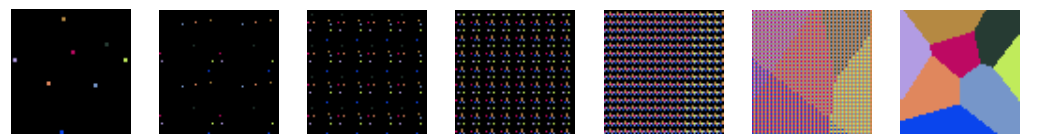
\includegraphics[width=15cm]{jfa}
  \caption{JFA illustration.}
\end{figure}


\paragraph{Discussion}
\par JFA (or JFA+1) is not optimal for the Voronoi map/Distance transformation problem. However, each jump can be implemented in a fine grain parallelism framework: during step $k$, each pixels can be processed in parallel (4 pixels are read and there is a final write). Hence, JFA is perfect for implementations on GPU where each
parallel core runs on texture map pixels (roughly). Note that optimal algorithm discussed in the lecture requires 1D propagation which could be tricky to implement on such GPU model.


% ----------------------------------------------------------------------
\section*{Exercise 2 \rm Lloyd's Relaxation}

\par In this exercise, we implement Lloyd's relaxation (also called $k-$means algorithm).  In many computer graphics applications, Lloyd's relaxation is widely used in order to ``uniformize'' point distributions.

The brute-force process is quite simple:
\begin{enumerate}
	\item Throw $N$ random points in the domain
	\item Compute the Voronoi map (here using JFA)
	\item For each cell:
	\begin{itemize}
		\item Compute its barycenter
		\item Move the corresponding site to the barycenter
	\end{itemize}
	\item Goto step 2 until ``stability''
\end{enumerate}

\par Beside this naive description, Lloyd's relaxation is related to an explicit energy function with many links to several fields (geometry processing, data-mining, \ldots). The convergence in the continuous plane can be obtained and the limit point distribution has many interesting properties.

\bigskip
{\bf Question} Implement the Lloyd's relaxation and at each step, output the site map.

\bigskip
\par You should observe that starting from uniform point distribution, the point set tends to a low discrepancy point distribution (points cover uniformly the space) and later toward hexagonal structures. At this point, the \emph{stability} criterion could just be a number of steps in the iterative process.

\par An example of the Lloyd's approach can be seen here: \url{http://www.youtube.com/watch?v=S0sAnabdCLg}



\end{document}
